\documentclass[a4paper,12pt,spanish,notitlepage]{report}
\usepackage[spanish]{babel}
\usepackage{graphicx}
\usepackage[utf8x]{inputenc}
\usepackage{color}
\usepackage{hyperref}
\usepackage{tikz}
\usepackage[all]{hypcap}
\usepackage[section]{placeins}
\renewcommand{\ttdefault}{lmtt}
\usetikzlibrary{calc,trees,positioning,arrows,chains,shapes.geometric,%
    decorations.pathreplacing,decorations.pathmorphing,shapes,%
    matrix,shapes.symbols}
\tikzset{
>=stealth',
  punktchain/.style={
    rectangle, 
    rounded corners, 
    % fill=black!10,
    draw=black, very thick,
    text width=10em, 
    minimum height=3em, 
    text centered, 
    on chain},
  line/.style={draw, thick, <-},
  element/.style={
    tape,
    top color=white,
    bottom color=blue!50!black!60!,
    minimum width=8em,
    draw=blue!40!black!90, very thick,
    text width=10em, 
    minimum height=3.5em, 
    text centered, 
    on chain},
  every join/.style={->, thick,shorten >=1pt},
  decoration={brace},
  tuborg/.style={decorate},
  tubnode/.style={midway, right=2pt},
}
\def\etc{\textsl{etc}}
\def\eg{\textsl{eg.}\ }
\def\etal{\textsl{et al.}}
\renewcommand\quote[1]{\lq\textsl{#1}\rq}
\newcommand\fr[2]{{\textstyle\frac{#1}{#2}}}
\def\name{\textsl{Ni intento Entertainment Kernel}}

\begin{document}
\title{\name\\\large\textit{Un kernel emulador}}
\author{Martín Villagra}
\maketitle
\vspace{1cm}
\centering{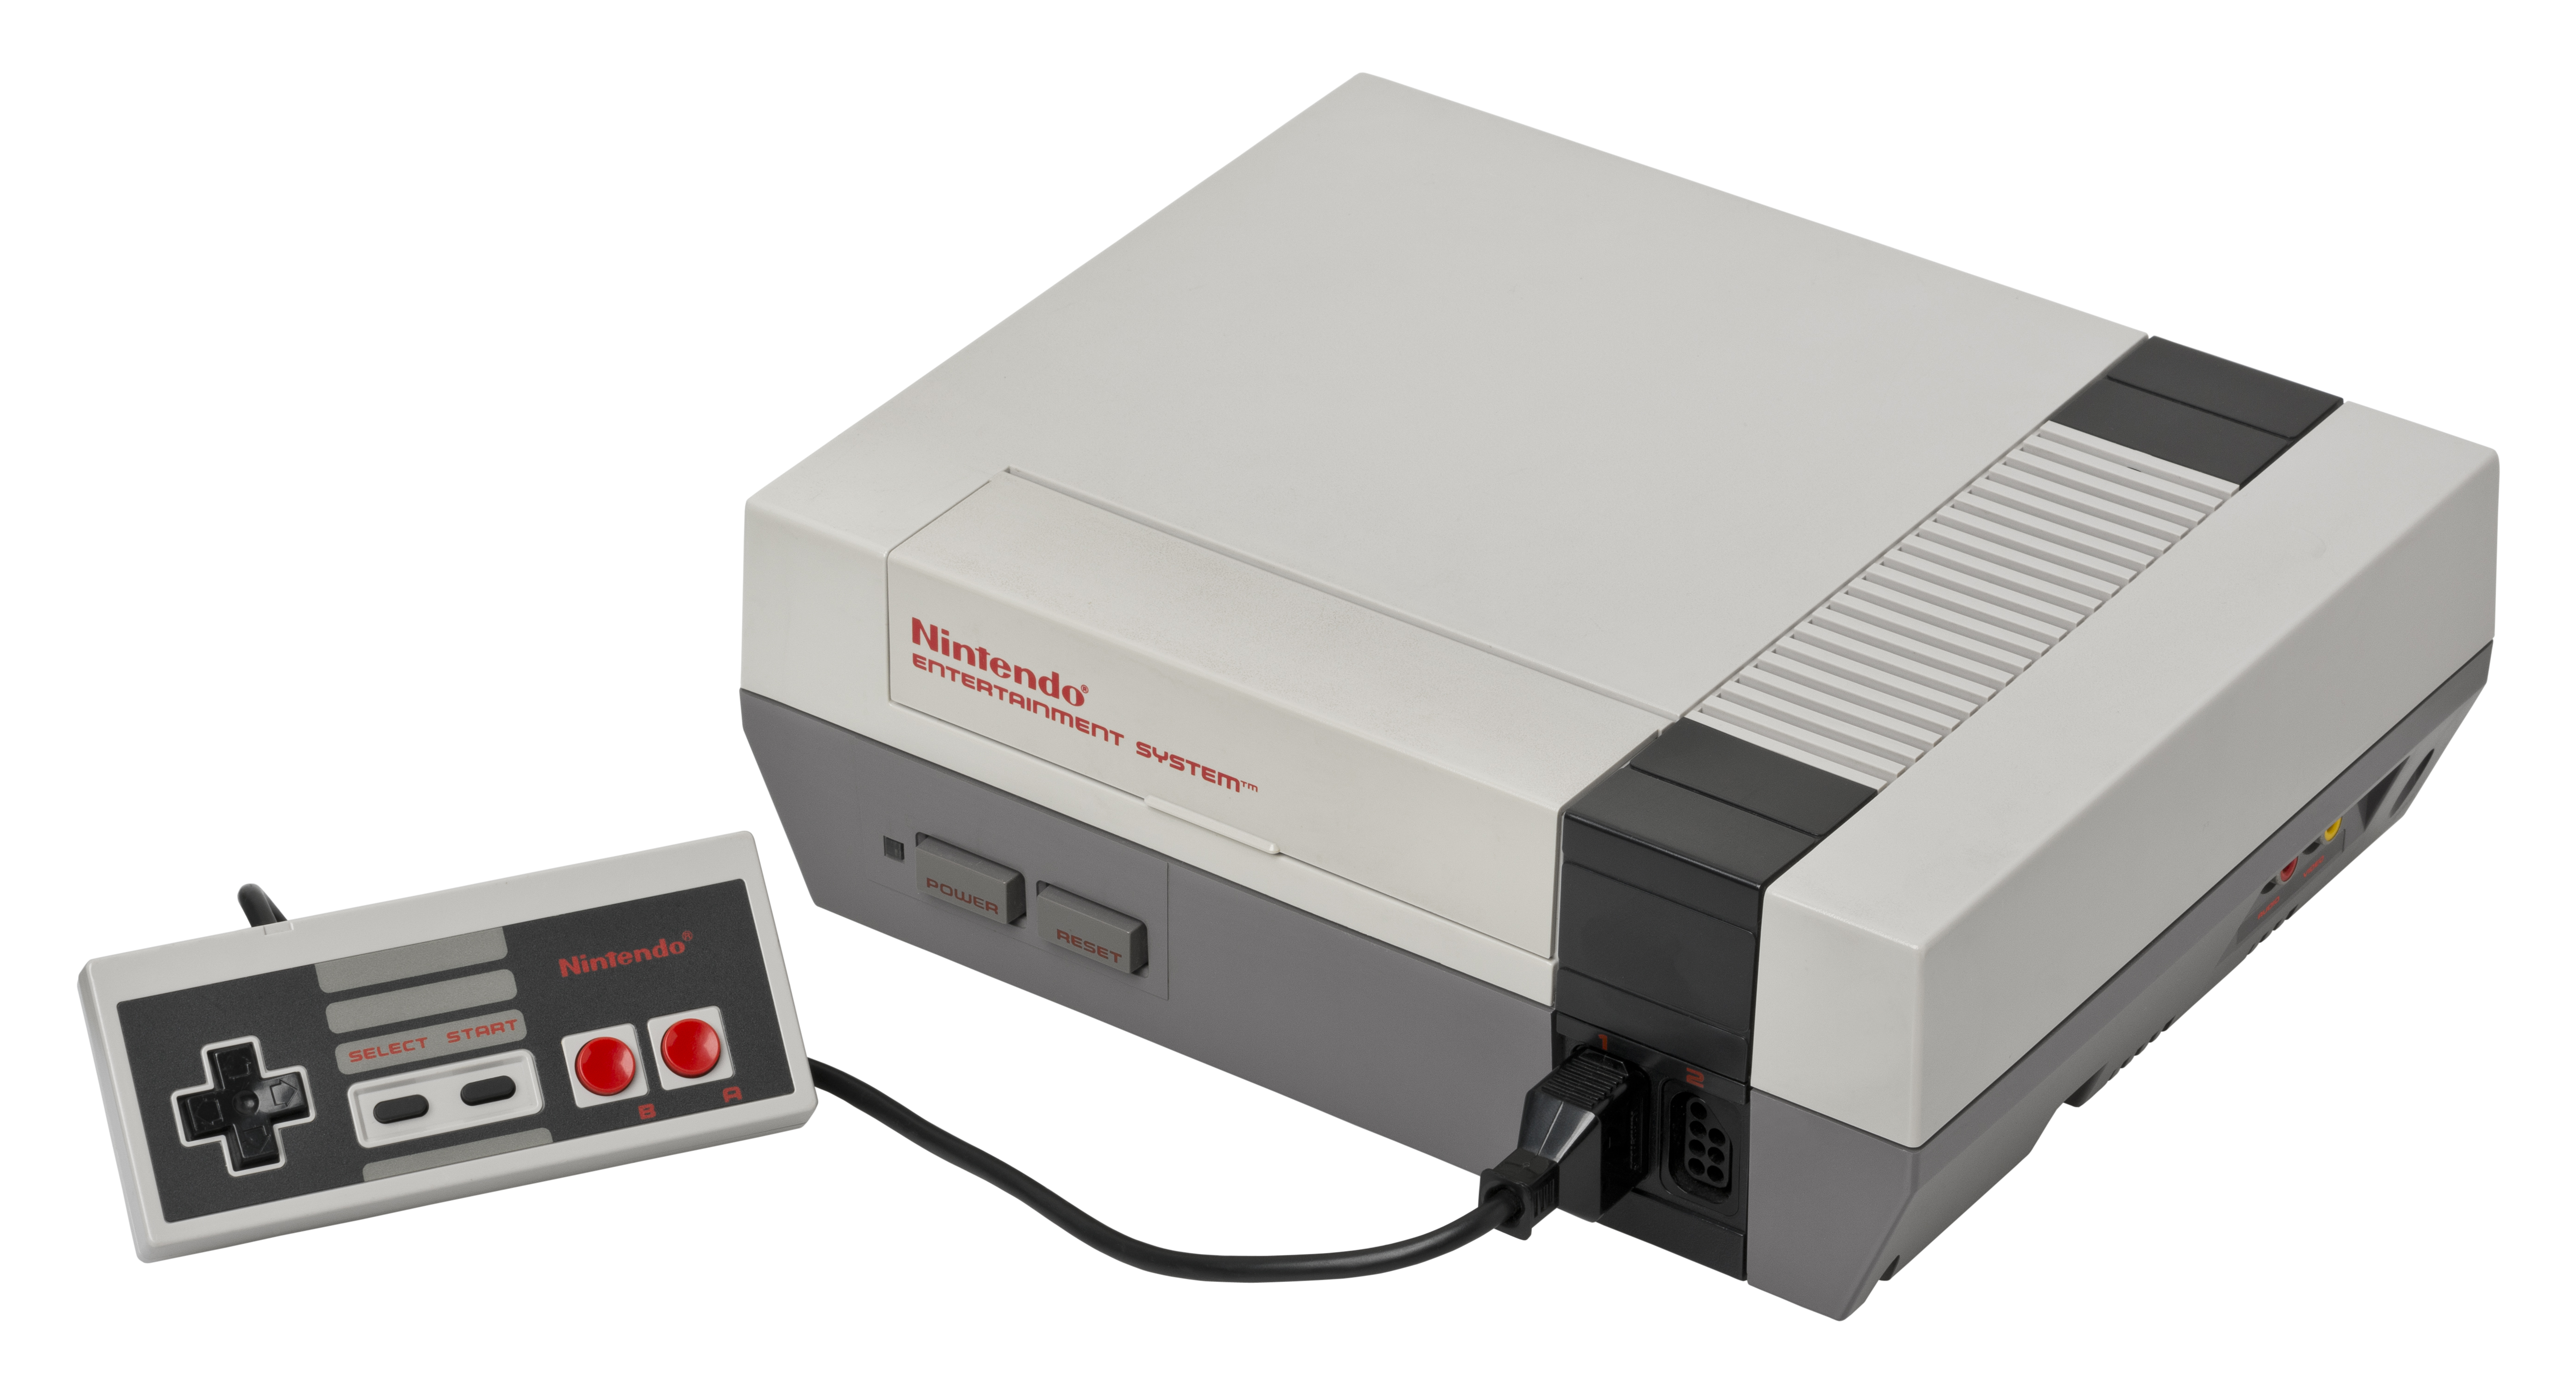
\includegraphics[width=\linewidth]{NES-Console-Set.jpg}}
\vspace{\fill}
\begin{abstract}\centering
El objetivo del trabajo es construir un emulador de la videoconsola Nintendo Entertaiment System(también conocida como Family) que se ejecute sin ningún sistema operativo de por medio.
\end{abstract}
\raggedright
%-----------------------------------------------------------
\tableofcontents
%-----------------------------------------------------------
\chapter{Introducción}
La consola NES\footnote{\url{http://en.wikipedia.org/wiki/Nintendo_Entertainment_System}}fue una de las consola más vendidas de todos los tiempos. En 2009, la misma fue nombrada la mejor consola de videojuegos de la historia por IGN\footnote{\url{http://uk.ign.com/top-25-consoles/1.html}}.
Gracias a su popularidad y simplicidad muchas personas se interesaron en el funcionamiento de la consola, dando lugar a una abundante documentación al respecto.

Fue por estas dos razones que se dicidió emular está consola en particular.

Por otro lado, se eligió realizar un kernel para no depender de ningún sistema operativo. Esto introduce la posibilidad de ejecutar el emulador en máquinas más restringidas, que obviamente resultarían de menor costo que una computadora o la consola original.

Debido a la gran extensión del trabajo, se decidió seguir la filosofía de no reinventar la rueda. El proyecto se construyó tomando como base otros kernels y emuladoras ya existentes.

\section{Estructuración}

En un principio dividimos en dos partes principales el projecto.

Una es el \textbf{emulador} propiamente dicho, es decir la que se encarga de hacer todo lo que hacía internamente la consola.

La otra parte es el \textbf{kernel} encargada de inicializar todo lo necesario para que el emulador funcione, así como proveerle funciones de bajo nivel tales como escribir en pantalla o reservar memoria. Al no tener un sistema operativo detrás, funciones como malloc y free que cualquier programador de C supone siempre presentes deben ser implementadas por el kernel.

\def\kernel{\textbf{kernel} }
\def\SO{\textbf{kernel} }
\chapter{El Kernel}

Un \kernel (de la raíz germánica Kern, núcleo, hueso) se define como la parte que se ejecuta en modo privilegiado (conocido también como modo núcleo), es decir con acceso irrestricto a todo el hardware del sistema. Es el principal responsable de facilitar a los distintos programas acceso seguro al hardware de la computadora y de  gestionar recursos.

En su más simple escencia es simplemente un código ejecutable, el cual es generado con un compilador como cualquier otro. La diferencia es que no tiene dependencias con librerías del sistema, tales como stdio.h o stdlib.h.

\section{Carácteristicas}
Empecemos por decir que lo que aquí se presenta está muy lejos de un sistema operativo completo. Se priorizó la simplicidad recortando todo lo que estaba de más, reduciendo al mínimo las capacidades del sistema. Por ejemplo la mayoría de los sistemas operativos pueden leer un programa y ejecutarlo. Nuestro querido kernel carece de esa posibilidad. A continuación se enumeran las carácteristicas principales del sistema.

\begin{itemize}
\item Dentro de la familia de arquitecturas x86\footnote{\url{http://en.wikipedia.org/wiki/X86}} se eligió i686\footnote{\url{http://en.wikipedia.org/wiki/P6_(microarchitecture)}}. Se prefirió esta por sobre x86\_64\footnote{\url{http://en.wikipedia.org/wiki/X86-64}} ya que tiene esta última no es soportada nativamente por GRUB(ver sección ~\ref{sec:booteo}). Respecto al formato de los ejecutables se eligió el que implementan los sistemas Unix\footnote{\url{http://en.wikipedia.org/wiki/Unix}}(como Linux\footnote{\url{http://en.wikipedia.org/wiki/Linux}}), el ELF \footnote{\url{http://en.wikipedia.org/wiki/Executable_and_Linkable_Format}}.
\item Es un kernel \underline{monolítico}, esto significa que todos los drivers y los servicios necesarios para el funcionamiento completo del sistema están incluídos en dentro del mismo kernel. Sistemas operativos como Linux no siguen esta filosofía, ya que implicaría cargar todos los drivers al incio del sistema, el cual tiene un costo de memoria muy alto. Esto no representa un problema para nosotros puesto que la cantidad de drivers y servicios ofrecidos por el kernel es muy reducida.
\item \underline{Monotarea}: Solo puede realizar una tarea a la vez, en nuestro caso el emulador. Para simplificar aún más incluso, el emulador es verdaderamente la \emph{única} tarea que el kernel puede ejecutar. Podría verse al emulador como un solo programa standalone, que no necesita ningún sistema operativo para ejecutarse.
\item Sin \underline{memoria virtual}: En un sistema operativo clásico cada proceso tiene sus propio mapa de direcciones virtuales. A medida que el proceso va solicitando más memoria se busca espacio en la memoria física y luego se le asigna la encontrada a una dirección virtual, la cual es usable por el proceso. Este sistema tiene ventajas tales como la posibilidad de restringir la memoria accesible por un proceso. Es destacable que la memoria física no tiene porque restringirse solo a la RAM\footnote{Random Access Memory}, puede apuntar incluso a una posición en el disco duro. Optamos por no incluir esta opción, para simplificar el sistema. Esto significa que los punteros contienen la dirección de memoria física y que es posible acceder y leer la memoria usada por otros procesos libremente.
\item Sin \underline{userspace}: Normalemente un sistema operativo puede dividirse en tres capas de abstracción diferentes, el hardware, el kernel y finalmente el userspace, que es donde se ejecutan las aplicaciones como Chromium, Notepad, \etc.
\end{itemize}
\begin{figure}[h]
\centering
\def\svgwidth{5cm}
\input{Kernel_Layout.pdf_tex}
\caption{Layout estándar de un kernel.}
\end{figure}
\FloatBarrier
En nuestro caso no tenemos userspace: el emulador, nuestro único programa a ejecutar, está embebido en el mismo kernel. Esto simplifica enormemente el diseño del kernel.

\section{Funciones}
Antes de hacer el kernel, hay que tener muy en claro que es exactamente lo que tiene que hacer. Surge la pregunta entonces ¿Qué necesita como mínimo nuestro emulador? Se muestra, en orden de importancia:
\begin{itemize}
\item Iniciar el sistema y ejecutar el emulador. Ver sección ~\ref{sec:booteo}.
\item Modificar libremente pixeles de la pantalla
\item Detectar pulsaciones del teclado
\item Poder reservar memoria dinámica *explicar que es*
\item Cargar de alguna forma los juegos
\item Ejecutar sonido
\item Escribir en algún medio persistente el estado actual del juego(Guardar la partida)
\end{itemize}
Pues bien, el kernel tiene que ser capaz de proveer funciones que faciliten cada una de estas tareas. En las siguientes secciones se detallaran cada una de ellas.

\section{Booteo}\label{sec:booteo}
*explicar que es un bootloader y la bios muy brevemente*
Para evitar tener que lidiar con la BIOS y otras interfaces de bajo nivel, se eligió utilizar un bootloader ya existente y ampliamente usado: GRUB. *poner que carajos es GRUB*. En particular existe un standard llamado Multiboot\footnote{\url{http://en.wikipedia.org/wiki/Multiboot_Specification}} que especifica como estructurar un kernel para que el mismo pueda ser cargado por GRUB(o por cualquier otro bootloader que implemente Multiboot). En particular se debe elaborar un header al inicio del kernel. En esta cabecera se determina por ejemplo que modo se prefiere(texto o consola) y que función va a ser la primera en ser llamada. A su vez GRUB se comunica con la BIOS entre otras cosas y recolecta información de la máquina que luego es recibida convenientemente por nuestro kernel. De esta forma al encender la máquina se iniciará GRUB, el mismo va a poder detectar nuestro kernel y lo va a ejecutar.

\subsection[boot.s]{boot.s\protect\footnotemark{}\protect\footnotetext{Ubicado en kernel/arch/x86/generic/init/boot.s}}
El problema es que al momento en que GRUB ejecuta el kernel el stack pointer no está inicializado por lo que no es posible que la función inicial sea en C. Debemos comenzar en assembler, inicializar el stack pointer y ahí si pasar a C. Esta es la razón de la existencia del archivo boot.s, que contiene el comienzo de nuestro kernel. Allí se incluye el header de Multiboot, el espacio para el stack y una función, la primera en ser llamada al iniciar el sistema, que inicializa el stack pointer y llama a nuestra función kernel\_entry\footnote{Ubicado en kernel/arch/x86/generic/init/kernel\_entry.c}(ya en C) que continua con la inicialización del sistema.

%-----------------------------------------------------------
\end{document}
